\section{Реализация}
\subsection{Архитектура и модель данных}
Приложение использует Jakarta EE 10: CDI управляет компонентами бизнес-логики, Jakarta REST обслуживает API, Jakarta Persistence и EclipseLink работают с PostgreSQL. Пользовательский интерфейс реализован средствами HTML, CSS и JavaScript. Транзакции имеют тип \texttt{RESOURCE\_LOCAL}; их границы заданы программно через \texttt{EntityTransaction}. Аннотация \texttt{@Transactional} в данной реализации не используется.

К существующим сущностям добавлены \texttt{ImportOperation}, состояния \texttt{RUNNING}, \texttt{SUCCESS}, \texttt{FAILED} и роли \texttt{USER}, \texttt{ADMIN}. История связана с учётной записью по идентификатору. В API возвращается безопасное представление: идентификатор операции, пользователь, статус, число добавленных фильмов только при успехе, время, имя файла и краткая причина ошибки. Пароли, соли и хеши в него не входят.

Миграция \path{003_lab2_roles_imports.sql} сохраняет существующие строки и назначает прежним пользователям роль USER. Повторное выполнение безопасно. Регистрация всегда создаёт обычного пользователя; роль администратора назначается серверным скриптом по точному имени уже зарегистрированной учётной записи.

\subsection{Формат импорта и проверка данных}
Файл передаётся на сервер как \path{multipart/form-data}, поле \texttt{file}, тип содержимого \path{application/json}. Браузер отправляет исходный объект File без преобразования JSON в JavaScript Number. Сохраняются Session Cookie и защита CSRF. Приняты ограничения 5 MiB и 1000 фильмов; пустой массив запрещён.

Верхний объект содержит целочисленный \texttt{formatVersion=1} и массив \texttt{movies}. Coordinates, Person и Location задаются вложенными объектами той же записи. Парсер проверяет UTF-8, допускает начальный BOM, отклоняет неизвестные и повторные свойства, автоматически формируемые поля, неверные типы, дробные значения целых полей, переполнение и неконечные числа. Long разбирается точно из целого JSON или десятичной строки; значение 9007199254740993 не проходит через Double. После разбора выполняется та же Bean Validation, что и при CRUD.

Для каждой записи создаются новые координаты. Человек определяется по уникальному \texttt{passportID}. Если человек уже существует, все его переданные поля должны совпадать; Location сравнивается по значениям, ZonedDateTime --- с учётом часового пояса, числа --- после преобразования в соответствующий Java-тип. Несовпадение вызывает \texttt{PERSON\_DATA\_CONFLICT}; импорт никогда не редактирует существующего человека неявно.

\subsection{Новая уникальность}
Бизнес-ключ имеет два независимых компонента: точное сохранённое название и \texttt{Person.id} режиссёра либо null. Регистр, пробелы и Unicode не нормализуются. Одноимённые люди с разными идентификаторами являются разными режиссёрами. Два фильма с одинаковым названием и отсутствующим режиссёром считаются дубликатами. Изменение имени или паспорта человека не меняет его идентификатор.

\texttt{MovieUniquenessValidator} используется обычным созданием, частичным обновлением и импортом. Обновление сначала объединяет входные поля с существующей сущностью и исключает собственный ID из поиска. Сравнение названия через Java String.equals обеспечивает точную семантику. Для нового сочетания в PostgreSQL отсутствуют UNIQUE, уникальные индексы и триггеры; прежние ограничения паспорта и имени пользователя сохранены.

\subsection{Транзакции и обработка отказов}
После проверки аутентификации, CSRF, наличия, размера и типа файла короткая транзакция T1 сохраняет RUNNING. Затем сервер разбирает файл. Транзакция T2 сначала блокирует строку \texttt{AppState(id=1)} через \texttt{PESSIMISTIC\_WRITE}; все окончательные чтения, проверки версий и уникальности выполняются после получения этой блокировки. Все вложенные объекты и фильмы сохраняются в T2. SUCCESS и фактическое число фильмов фиксируются в той же транзакции; revision увеличивается один раз.

При ошибке T2 полностью откатывается. Независимая транзакция T3 сохраняет FAILED с пустым addedCount; история не исчезает вместе с объектами. Исторические транзакции не изменяют revision. Flush не является commit. Это существенно при IDENTITY: фактические INSERT могут выполняться до конца обработки файла, но остаются частью одной транзакции.

При неопределённом исходе commit новая связь с БД сначала проверяет историю. Уже подтверждённый SUCCESS не заменяется на FAILED. При недоступности проверки операция остаётся RUNNING; клиент получает идентификатор и указание проверить историю, без автоматической повторной загрузки. После остановки прежнего единственного экземпляра скрипт запуска проверяет процесс, получает блокировку AppState и восстанавливает оставшиеся RUNNING. Этот порядок предназначен для одного экземпляра приложения.

SQLSTATE 55P03, 57014 и известные временные ошибки отделены от бизнес-конфликтов; неожиданный сбой не выдаётся за допустимый 409. Для явно отменённых транзакций SERIALIZABLE предусмотрено не более трёх повторов с новым EntityManager. Пользовательские ошибки и конфликты версий не повторяются.

\subsection{Веб-интерфейс}
Добавлены страницы импорта и истории. Во время отправки повторный щелчок отключён; результат показывает ID операции, число фильмов либо код, номер записи и путь поля. История имеет собственный опрос, поэтому неуспешный импорт виден без изменения revision. Обычный пользователь видит свои операции, администратор --- все; проверка принадлежности выполняется сервером и для списка, и для отдельной записи.

По требованию пользователя итоговый интерфейс полностью русскоязычный; переключатель языка и номер варианта в верхней части страницы удалены. Механизм синхронизации первой работы сохранён: открытая форма оставляет пользовательский ввод и первоначальную версию, а сервер отклоняет устаревшее сохранение.

\section{UML-диаграммы}
Диаграммы отражают окончательные сущности и компоненты приложения. Редактируемые исходники Graphviz DOT, изображения SVG/PNG/PDF и контрольные суммы Java-файлов находятся в каталоге \path{report/Lab2/uml/}.

\begin{figure}[H]\centering
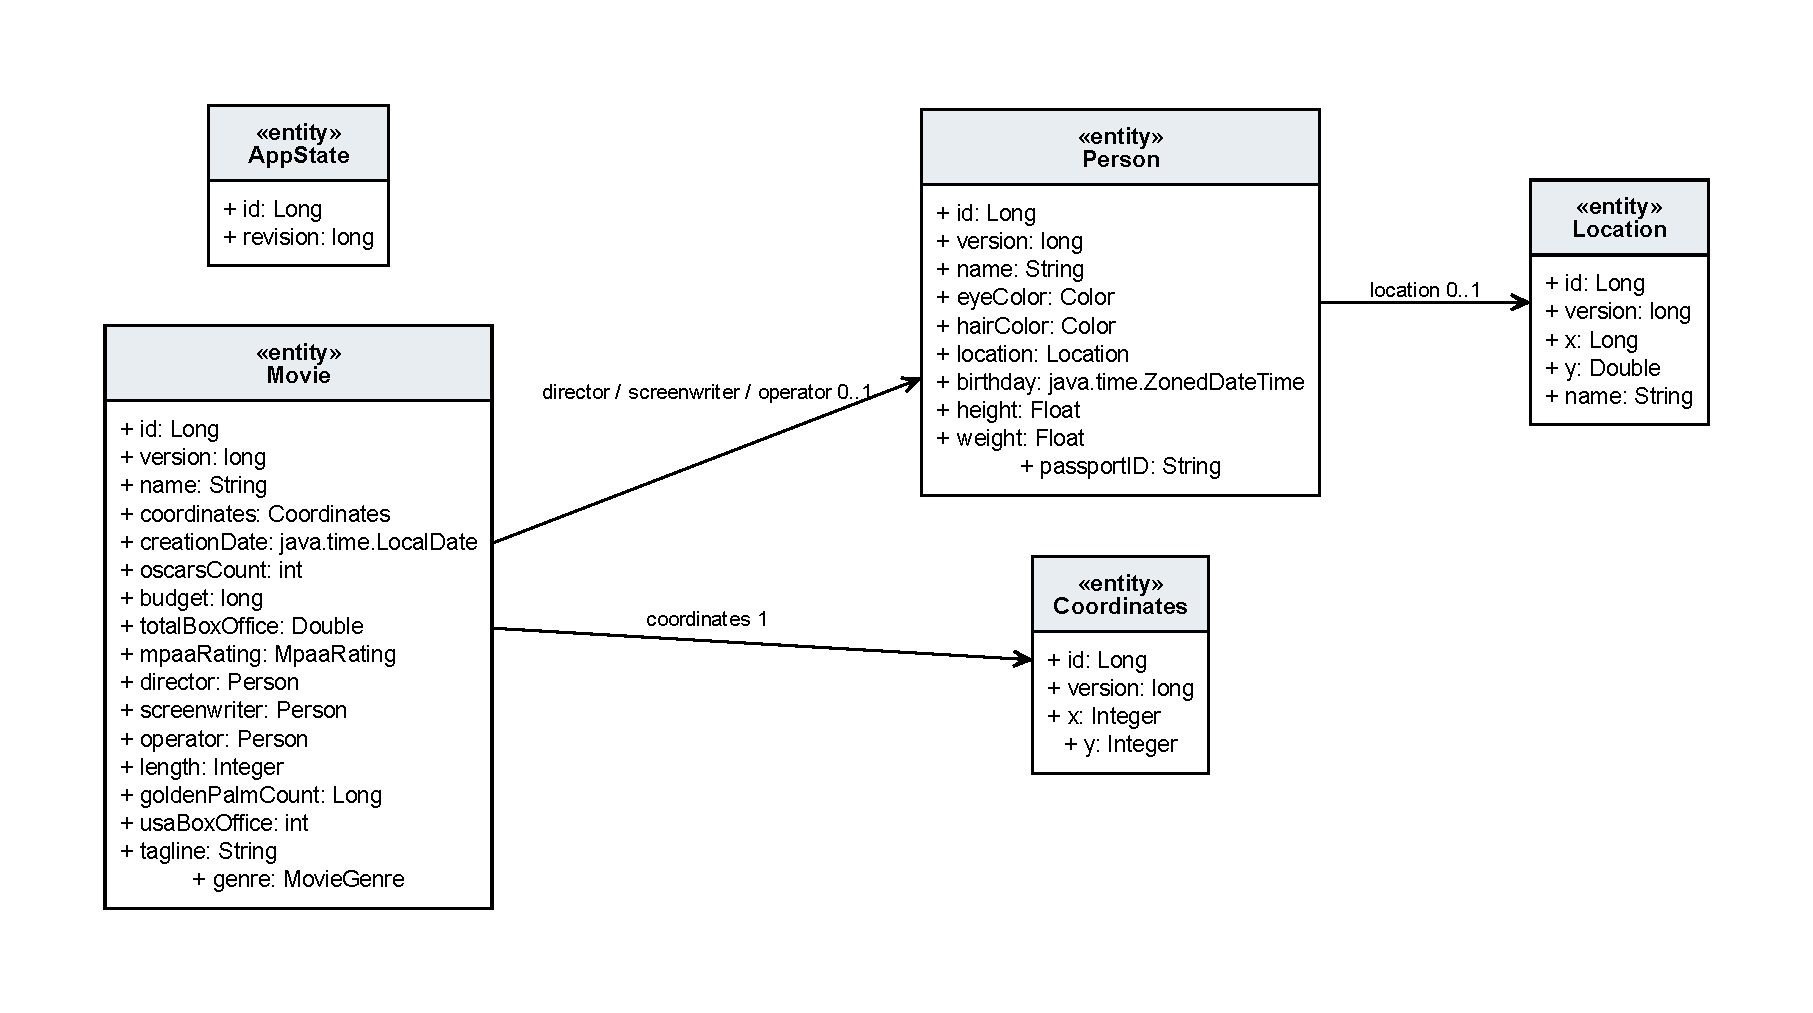
\includegraphics[width=\textwidth,height=0.72\textheight,keepaspectratio]{uml/classes-domain.pdf}
\caption{Классы предметной области и связи с вложенными объектами}
\end{figure}
\begin{figure}[H]\centering
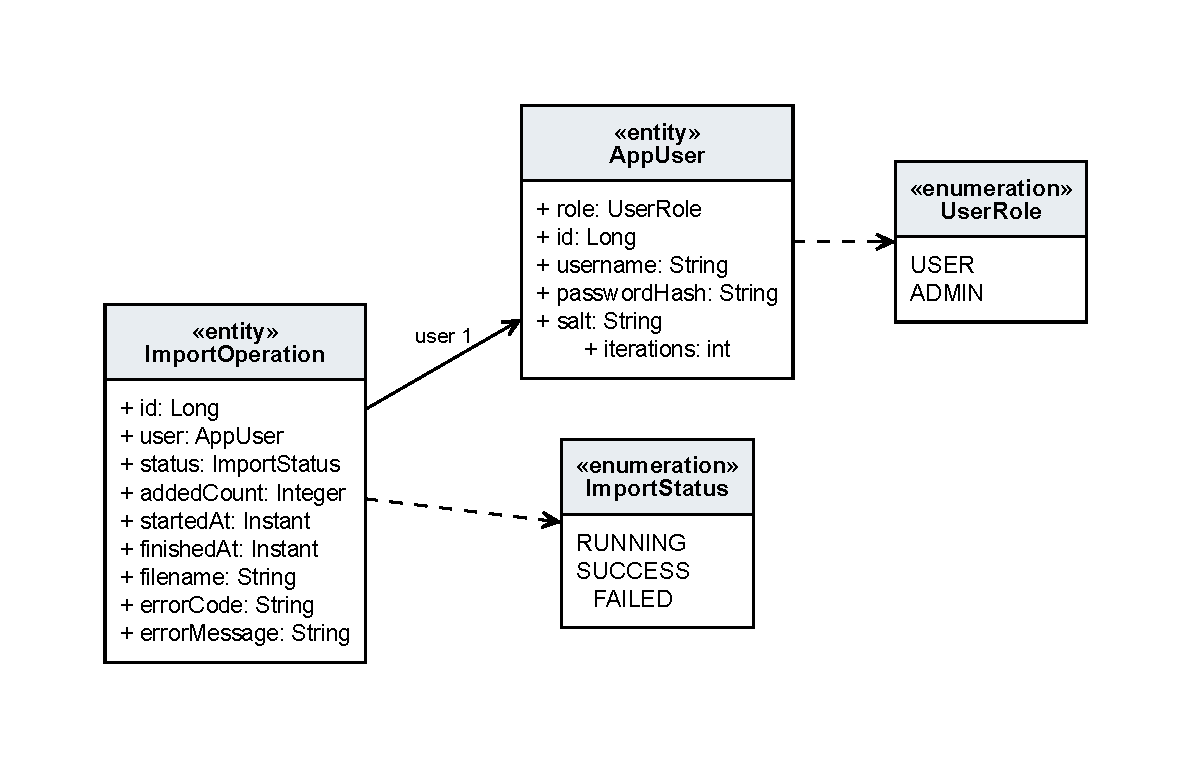
\includegraphics[width=\textwidth,height=0.65\textheight,keepaspectratio]{uml/classes-history.pdf}
\caption{Учётные записи, роли и устойчивое состояние импорта}
\end{figure}
\begin{landscape}
\begin{figure}[p]\centering
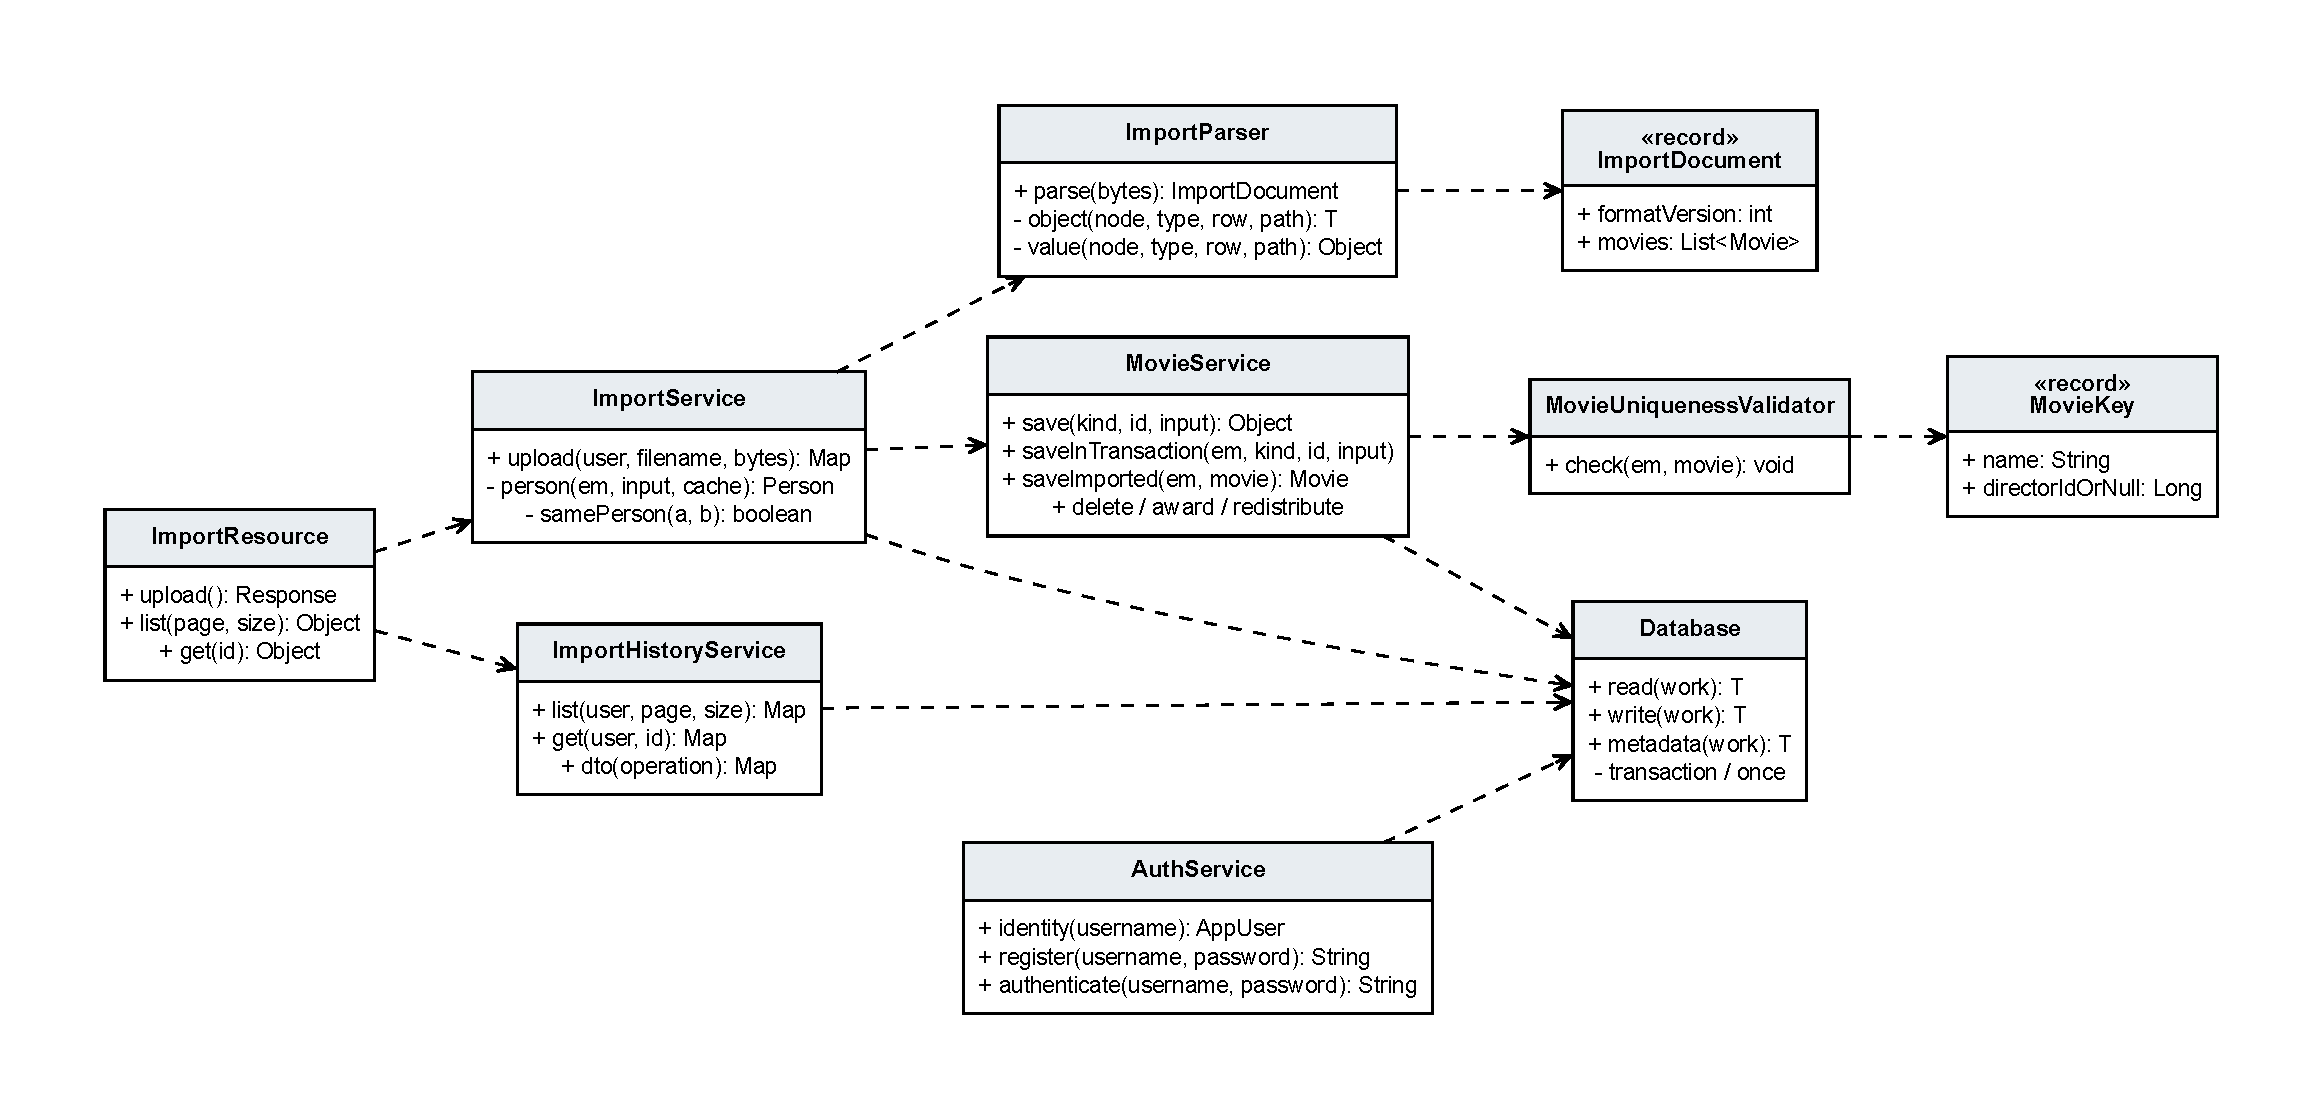
\includegraphics[width=\linewidth,height=0.85\textheight,keepaspectratio]{uml/classes-services.pdf}
\caption{Компоненты импорта, DTO и транзакционная граница}
\end{figure}
\end{landscape}
\begin{figure}[H]\centering
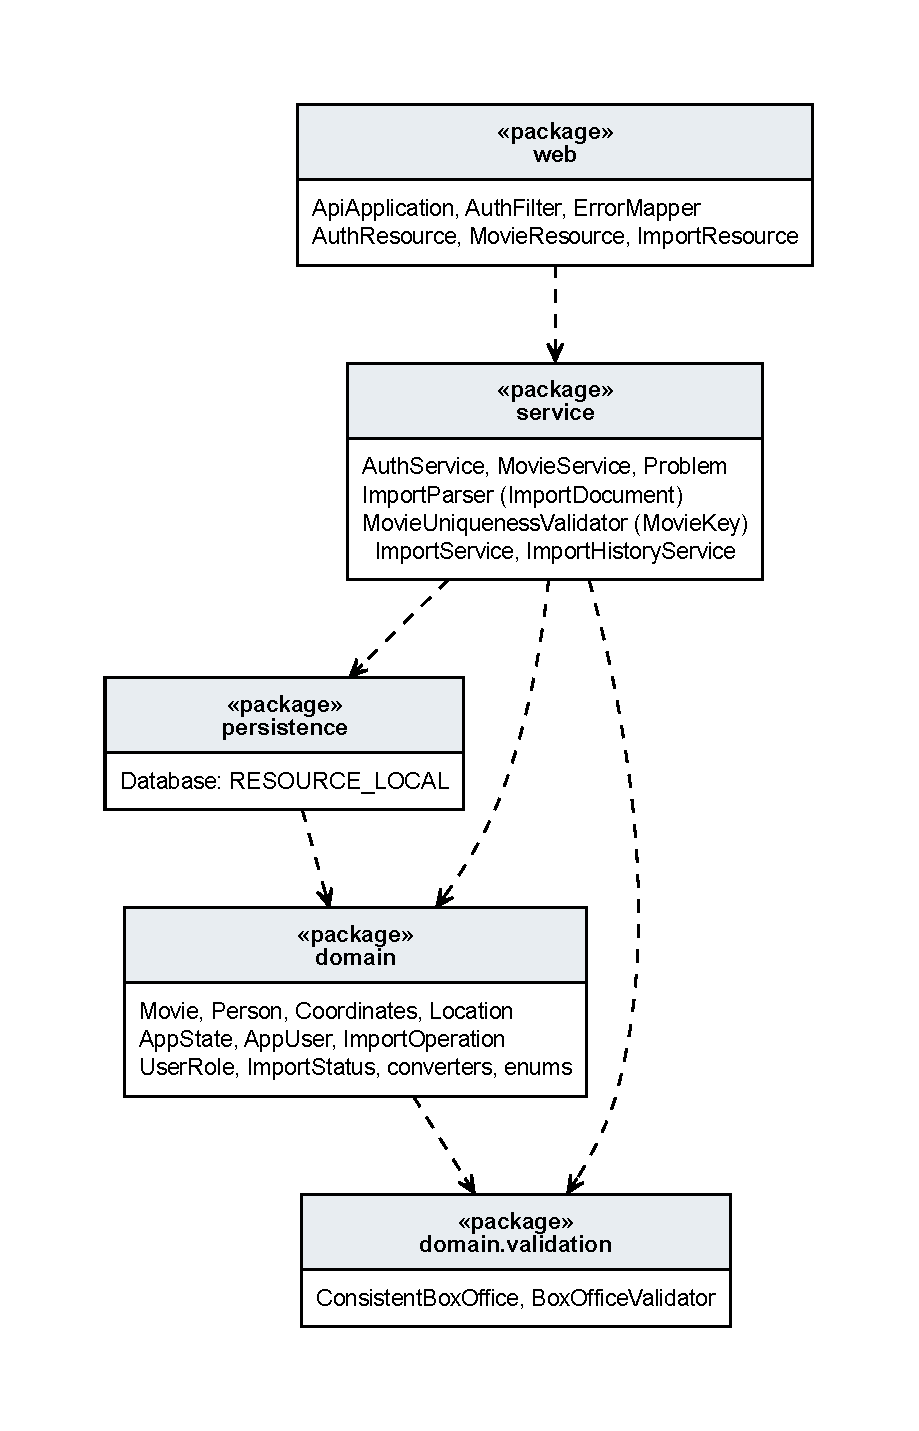
\includegraphics[width=\textwidth,height=0.65\textheight,keepaspectratio]{uml/packages.pdf}
\caption{Пакеты приложения и зависимости}
\end{figure}
